\chapter{Laboratory Results}\label{chap:Results}
This chapter presents test results obtained when applying continuous height, discrete time and action function approximation Q-Learning to the Smart Water Infrastructure Laboratory shown in \cref{fig:AAUSWIL}, which is used to emulate the small scale water distribution network presented in \cref{sec:WDNsetup}.

Due to long convergence times the control method implemented is based on the final approximated action value function obtained in \cref{sec:sim1D}. This means control will be based on simulation learning, such that we do not have to learn in the laboratory. Because we have to wait for water level changes to happen, along with long convergence times at thousands of iterations, learning would take weeks in the real world. The performance results when using simulated training, depends on the similarities between test setup and simulations.

There are known differences between test setup and simulation, simulations use a model which is not entirely accurate to simulate water level changes. To reduce experiment length, an hour is made equivalent to one minute in the test setup. This gives behaviour similar to a changed flow or changed cross sectional area of the reservoir, meaning the change of water level will be different.

The test setup does not allow separate pumps to run independently. However, they do have speed control. Therefore rotational speeds will be set equally on two pumps at three different speeds, resembling three different actions. The speeds are chosen to yield combined flows matching simulation flows as well as possible.

Test details:
\begin{itemize}
	\item \textbf{Run time:} 144 minutes - representing 144 hours/6 days in real life. Simulations use time increments of one hour, we use the same concept for laboratory test, however, one hour will be equivalent to 1 minute. Among many things, this means a new actions is chosen every minute, and water level changes due to that actions, occur over the next 60 seconds.\\
	
	\item \textbf{Consumer demand:} Periodic over a 24 minute interval. 24 minutes (96 samples) represent 24 hours of a real day. Demand corresponds to normalised profile showed in \cref{sec:Consumption}. Demand is sampled every 15th second. Flows resembling simulation flows are obtained by controlling a variable valve with a PI-controller with the consumer profile described in \cref{sec:Consumption} used as a reference.\\
		
	\item \textbf{Time state:} As in simulation, time is discretises into 24 states \cref{sec:WDNTabularQ-Learning} and \cref{sec:WDN1D}.	
		
	\item \textbf{Weight vector \textbf{w}}: is obtained from simulation in \cref{sec:sim1D} and have dimension: $ \mathbb{R}^{3 \times 24 \times 10} $ corresponding to 10 radial basis functions with centers placement described in \cref{sec:WDN1D} \\ 
	
	\item \textbf{Actions:} are percentage pump rotational speeds, which are matched to fit simulation flows through trial and error before running results. As such actions are equivalent to rotational speeds of 50\%,\ 65\% and 100\%.
	
	\item  \textbf{Initial conditions:} initial water level of 38cm at $t=1$.
\end{itemize}

\begin{figure}[h!]
	\centering
	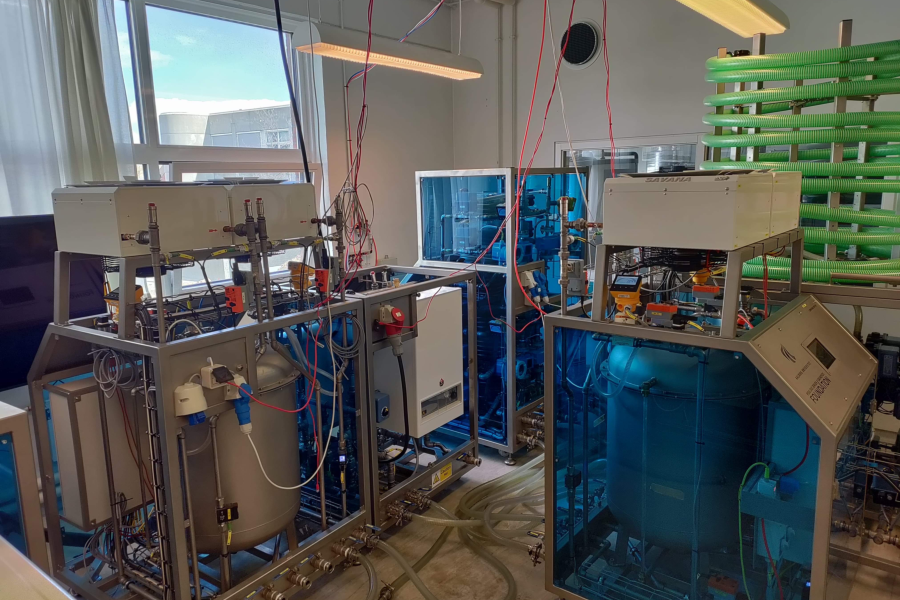
\includegraphics[width=0.7\linewidth]{Figures/SWIL.pdf}
	\caption{Picture of the AAU SWIL.}
	\label{fig:AAUSWIL}
\end{figure}

\clearpage

\section{Laboratory Setup}
\cref{fig:LabSetup} shows a diagram of the setup of laboratory modules. The pump station supplies water to the system, all water flows through a pipe module, both to add pipe length for a more realistic setup and to utilize the module's sensors. Water flows both to and from the elevated water reservoir. Flow to the consumer is regulated using a controllable valve in the module. Water is circulated using auxiliary pumps in the pump station. For a more detailed diagram of the setup, see Simulink setup in \cref{app:Simulink}. This diagram show simulink setup resembling the figure in this chapter, including specific names and numbers of the used sensors and  pumps.

\begin{figure}[h!]
	\centering
	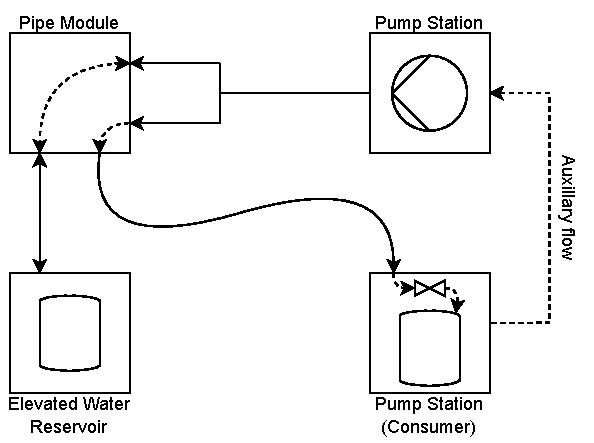
\includegraphics[width=0.7\linewidth]{Figures/LABsetupPDF.pdf}
	\caption{Diagram showing simple laboratory module setup.}
	\label{fig:LabSetup}
\end{figure}

\newpage

\section{Results}
\cref{fig:HtankResult} present the water level in the elevated water reservoir over a timespan of $ 144 $ minutes. Just like in \cref{chap:Simulation} a periodicity is visible in the water level, which is expected due to the periodicity in the consumer demand shown in \cref{fig:Consumption}. Water level is nicely reduced to the optimal value around 25 as expected similarly to simulation results in \cref{sec:sim1D}. The fact that the water level settles so far above the barrier in both simulation and laboratory is discussed in the following chapter. 

The simulated mean water level for the last five periods is $24.55$ and for laboratory results the mean is $25.25$, which we consider to be similar behaviour. The water level variance seems greater for laboratory results, likely because the demand is sampled four times more often, and demands are not as accurate as in simulation, since the demand is controlled via a valve which has a settling time.

\begin{figure}[h!]
	\centering
	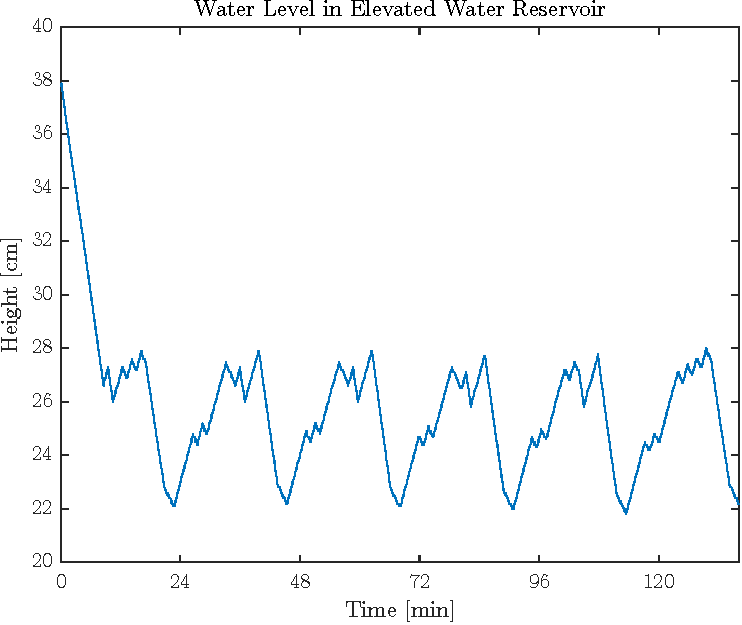
\includegraphics[width=0.7\linewidth]{figures/ResultHeight.pdf}
	\caption{Water level in elevated water reservoir, showing a period of 5 days.}
	\label{fig:HtankResult}
\end{figure}

The difference to simulation results was expected based on the already known differences between test setup and simulation. One of the advantages to reinforcement learning mentioned in this project is its ability to adapt to changes in the environment. However, this implementation does not include learning, due to Simulink implications. We are certain that a full reinforcement learning method with learning and exploration can be implemented in Simulink, but was not within scope of this project.

Furthermore, for the same reasons, this implementation does not include exploration. The nature of the Simulink issues are from storing previous values while the simulation is running. We do not see any reason that this should not be doable in Simulink if more time was available. 

\cref{fig:PumpResult} shows actions chosen by the reinforcement learning agent. A  periodic pump profile is visible as expected. Notice the lowest rotational speed is used as long as there is too much water in the reservoir.

\begin{figure}[h!]
	\centering
	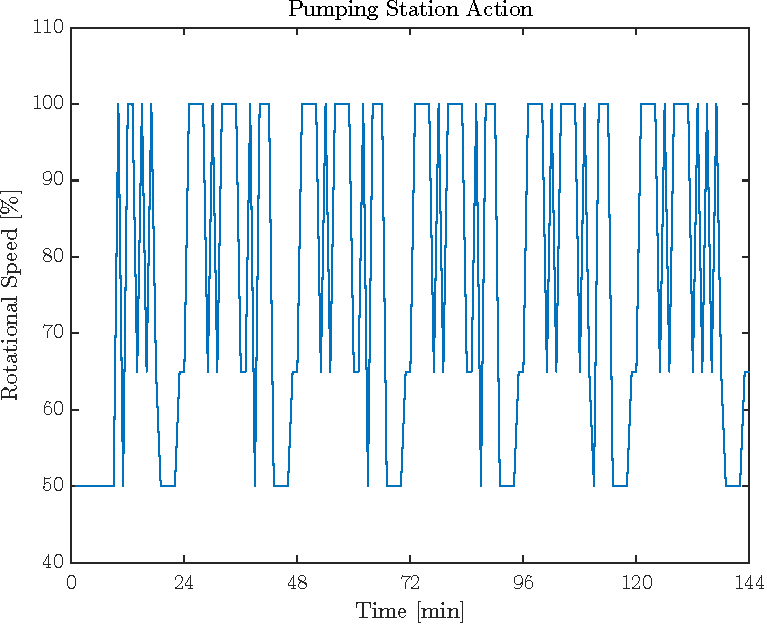
\includegraphics[width=0.7\linewidth]{figures/ResultPumpSpeed.pdf}
	\caption{Pump profile showing rotational speed (actions) over time.}
	\label{fig:PumpResult}
\end{figure}

